\begin{figure*}[t!]
\centering
% 45 for single column
\subfigure[$MGTCOM$ + $L_y$]{
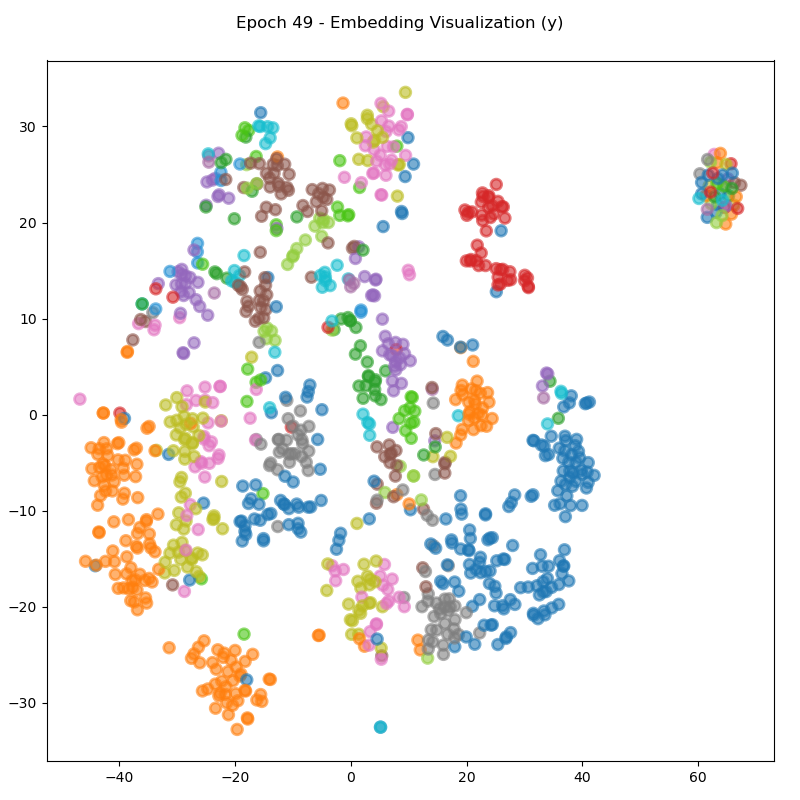
\includegraphics[width=0.23\columnwidth]{resources/visualization/combi_y.png}
}
\subfigure[$MGTCOM$ + $L_{\mathcal{T}}$]{
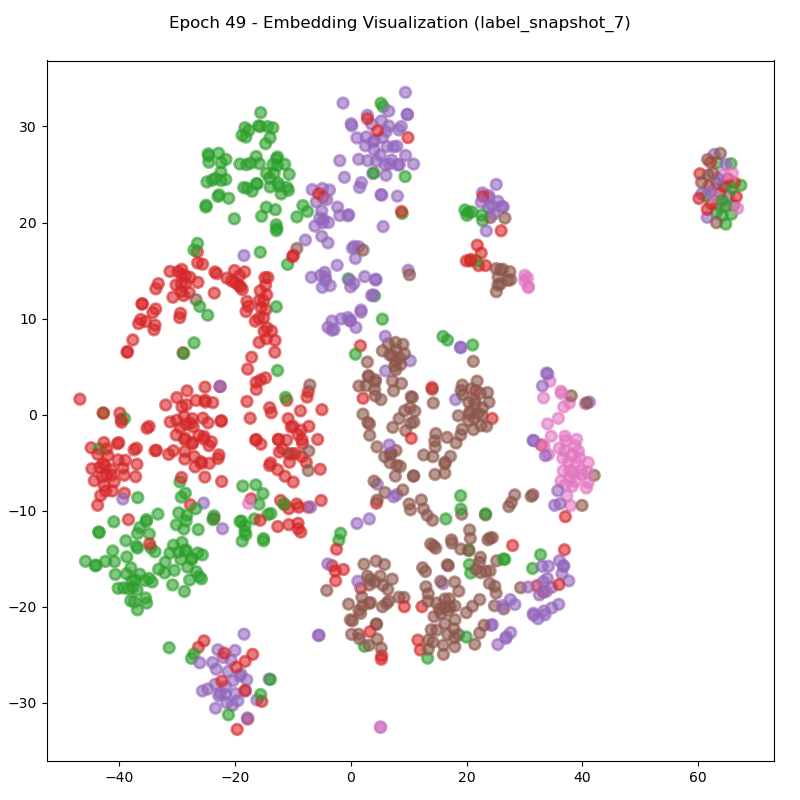
\includegraphics[width=0.23\columnwidth]{resources/visualization/combi_t.png}
}
\subfigure[$ComE$ + $L_y$]{
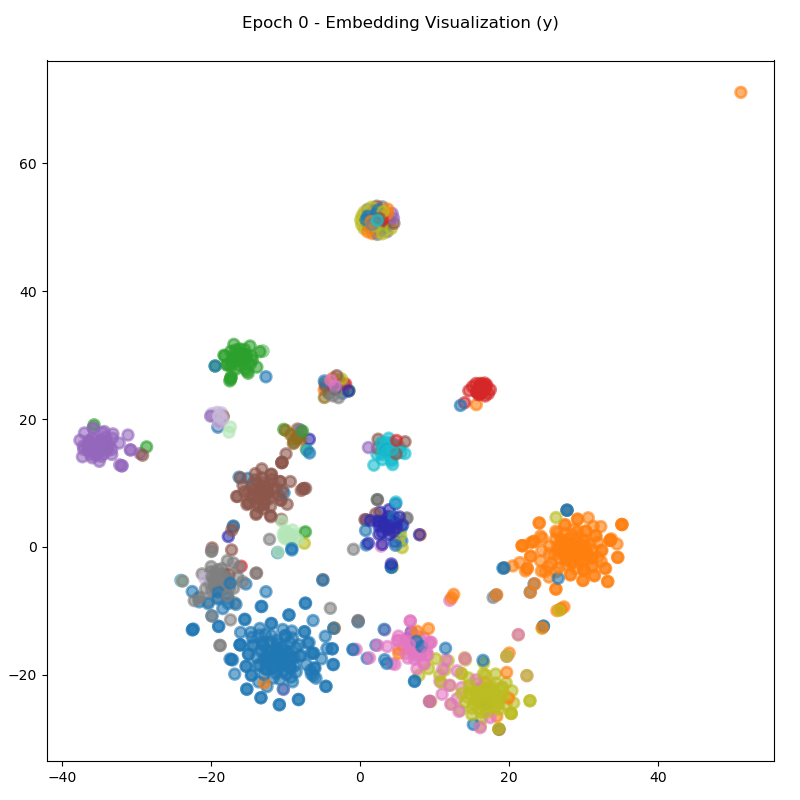
\includegraphics[width=0.23\columnwidth]{resources/visualization/come_y.png}
}
\subfigure[$ComE$ + $L_{\mathcal{T}}$]{
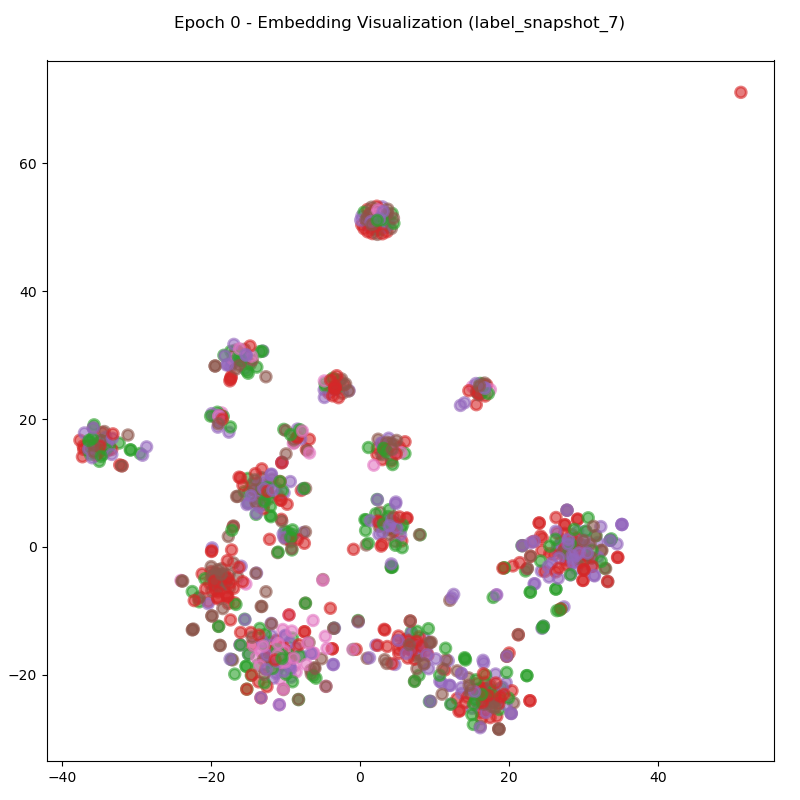
\includegraphics[width=0.23\columnwidth]{resources/visualization/come_t.png}
}\\

\centering
\subfigure[$Node2Vec$ + $L_y$]{
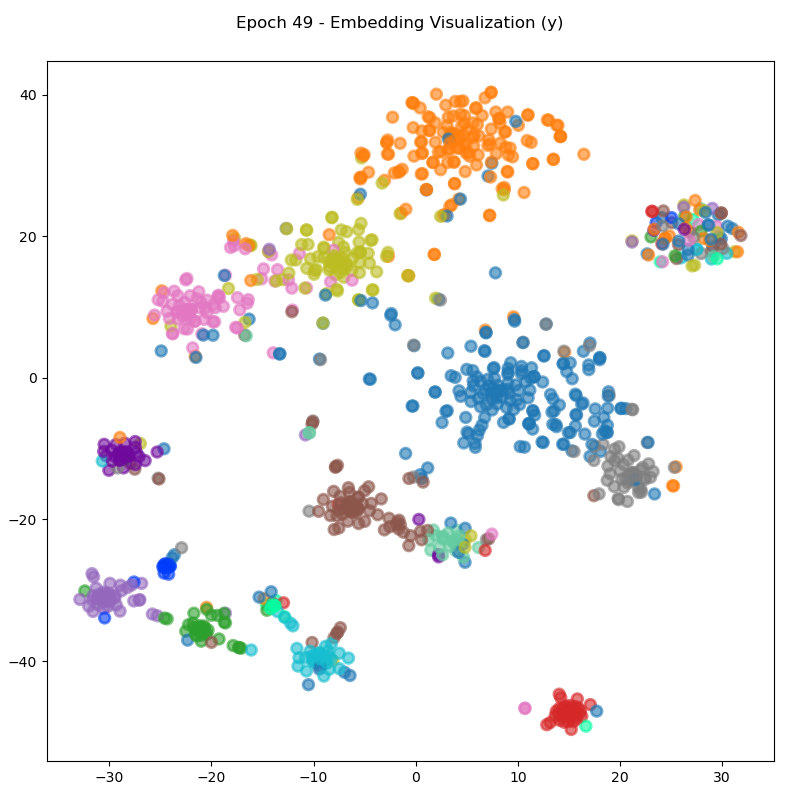
\includegraphics[width=0.23\columnwidth]{resources/visualization/n2v_y.png}
}
\subfigure[$Node2Vec$ + $L_{\mathcal{T}}$]{
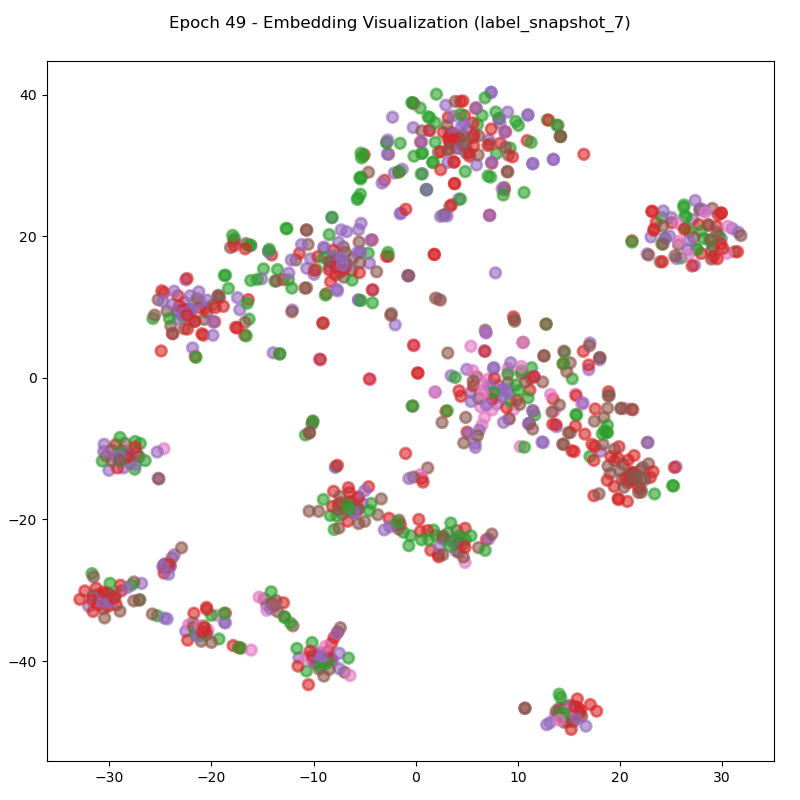
\includegraphics[width=0.23\columnwidth]{resources/visualization/n2v_t.png}
}
\subfigure[$CTDNE$ + $L_y$]{
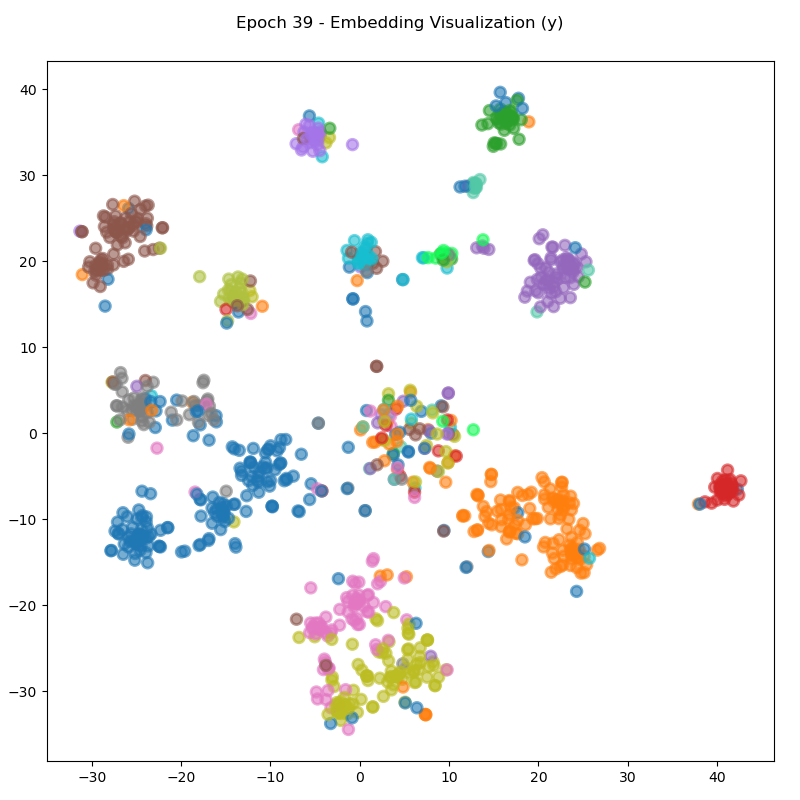
\includegraphics[width=0.23\columnwidth]{resources/visualization/ctdne_y.png} 
}
\subfigure[$CTDNE$ + $L_{\mathcal{T}}$]{
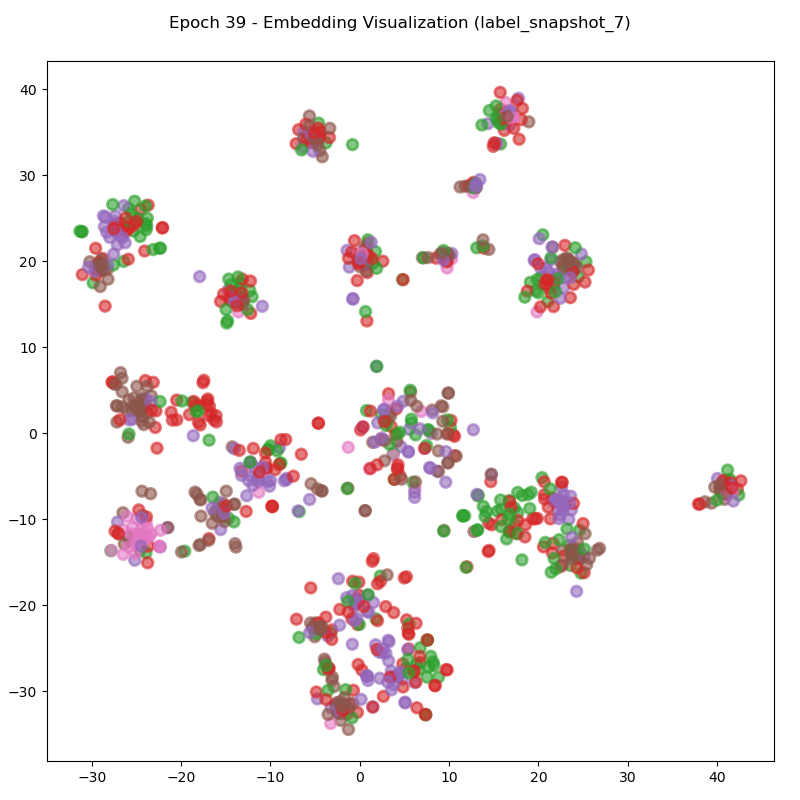
\includegraphics[width=0.23\columnwidth]{resources/visualization/ctdne_t.png}
}
\caption{Visualization of trained embedding against ground truth labels ($L_y$,  left) and timestamp labels ($L_{\mathcal{T}}$, right) for DBLP-HCN dataset.
(Note: The embeddings are calculated on the training dataset. Each of the plots contains a blob of nodes that have no edges in the training set due to the validation split. None of the methods is equipped to handle disconnected nodes.)
}
\label{fig:embeddings}
\end{figure*}    